\lecture{Geometria Analitica e trasformazioni nello spazio}{02~-~06~-~2026}
%
%
\section{Traslazioni e coordinate omogenee}
%
\subsection{Traslazioni} Sposta (trasla, disloca) un punto in una nuova posizione.
\begin{definition}
    Dislocazione di un punto $ p $ in una nuova posizione $ p' $ utilizzando un vettore di spostamento $ d $;
    \[
        p' = p + d
    \]
\end{definition}
\emph{Rappresenta tre gradi di libertà}.
%
\subsection{Coordinate omogenee}
Per rappresentare la traslazione si utilizza un sistema a quattro dimensioni (coordinate omogenee), dove un punto è rappresentato come:
\[
    p = \begin{bmatrix}
        x, y, z, 1
    \end{bmatrix}^{T}
\]
\[
    p'= \begin{bmatrix}
        x',y',z',1
    \end{bmatrix}^{T}
\]
e il vettore di traslazione come:
\[
    d = \begin{bmatrix}
        dx, dy, dz, 0
    \end{bmatrix}^{T}
\]
Questo permette di esprimere l'operazione come l'addizione tra un punto e un vettore.
\begin{definition}
    Possiamo quindi dire che $ p' = p + d $, oppure:
    \begin{align*}
        x' = x + d_{x} \\
        y' = y + d_{y} \\
        z' = z + d_{z}
    \end{align*}
    Da ricordarsi che:
    \begin{itemize}
        \item L'espressione è in \emph{4 dimensioni}, ed esprime punto = vettore + punto;
        \item Quando si parla ad esempio di $ x' = x + d_{x} $, ricordiamoci che per $ d_{x} $ si intende il \textbf{vettore d in x}, e non la derivata di x $ \frac{d}{dx} $.
    \end{itemize}
\end{definition}

%
\subsection{Matrice di traslazione}
La traslazione può essere espressa tramite una matrice $ 4 \times 4 $ di nome $ T $ in coordinate omogenee $ p'=Tp $ dove:
\[
    T = T \begin{pmatrix}
        d_{x}, d_{y}, d_{z}
    \end{pmatrix} = \begin{bmatrix}
        1 & 0 & 0 & d_{x} \\
        0 & 1 & 0 & d_{y} \\
        0 & 0 & 1 & d_{z} \\
        0 & 0 & 0 & 1
    \end{bmatrix}
\]
Questa forma è la preferita a livello implementativo perché permette di esprimere tutte le trasformazioni affini in questo modo e consente di concatenare facilmente trasformazioni multiple moltiplicando le matrici.

%
\section{Rotazioni in 2 e 3 dimensioni}
\begin{theorem}[Rotazioni in 2 dimensioni attorno all'origine]
    Si consideri una rotazione attorno all'origine di $ \theta $ gradi: il raggio resta uguale, l'angolo aumenta di $ \theta $.
    \begin{center}

        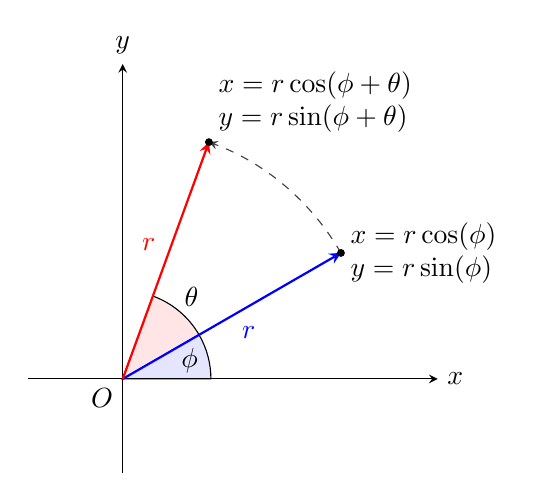
\begin{tikzpicture}[>=stealth, scale=.8]

            % 1. SFONDI COLORATI PER GLI ANGOLI (Disegnati per primi così non coprono le linee)
            % Angolo theta (colore rosso, raggio 1.4cm, da 30 a 70 gradi)
            \draw[fill=red!10, draw=black] (0,0) -- (30:1.4) arc [start angle=30, end angle=70, radius=1.4cm] -- cycle;
            \node at (50:1.7) {$\theta$};

            % Angolo phi (colore blu, raggio 1.4cm, da 0 a 30 gradi)
            \draw[fill=blue!10, draw=black] (0,0) -- (1.4,0) arc [start angle=0, end angle=30, radius=1.4cm] -- cycle;
            \node at (15:1.1) {$\phi$};


            % 2. ASSI CARTESIANI
            \draw[->] (-1.5,0) -- (5,0) node[right] {$x$};
            \draw[->] (0,-1.5) -- (0,5) node[above] {$y$};
            \node[below left] at (0,0) {$O$};

            % Parametri della rotazione
            \def\R{4}           % Lunghezza del raggio r
            \def\angPhi{30}     % Angolo iniziale phi
            \def\angTheta{40}   % Angolo di rotazione theta

            % Definizioni dei Punti
            \coordinate (O) at (0,0);
            \coordinate (P) at (\angPhi:\R);
            \coordinate (Pprime) at ({\angPhi+\angTheta}:\R);


            % 3. PROIEZIONI E LINEE TRATTEGGIATE
            % % Proiezioni per il punto P (x, y)
            % \draw[dashed, gray] (P) -- (P |- O) node[below, text=black] {$x$};
            % \draw[dashed, gray] (P) -- (O -| P) node[left, text=black] {$y$};

            % % Proiezioni per il punto P' (x', y')
            % \draw[dashed, gray] (Pprime) -- (Pprime |- O) node[below, text=black] {$x'$};
            % \draw[dashed, gray] (Pprime) -- (O -| Pprime) node[left, text=black] {$y'$};


            % 4. VETTORI E ARCO DI ROTAZIONE
            % Vettori (raggi r)
            \draw[->, thick, blue] (O) -- (P) node[midway, below right] {$r$};
            \draw[->, thick, red] (O) -- (Pprime) node[midway, above left] {$r$};

            % Arco tratteggiato che mostra il movimento della rotazione
            \draw[->, dashed, darkgray] (\angPhi:\R) arc [start angle=\angPhi, end angle={\angPhi+\angTheta}, radius=\R];


            % 5. ETICHETTE DEI PUNTI
            \filldraw (P) circle (1.5pt) node[right, align=left] {$x = r \cos(\phi)$ \\ $y = r \sin(\phi)$};
            \filldraw (Pprime) circle (1.5pt) node[above right, align=left] {$x = r \cos (\phi + \theta)$ \\ $ y = r \sin (\phi + \theta) $};

        \end{tikzpicture}
    \end{center}
    Le coordinate del nuovo punto si calcolano tramite le funzioni trigonometriche:
    \begin{align*}
        x' = x \cos \theta - y \sin \theta \\
        y' = x \sin \theta + y \cos \theta
    \end{align*}
\end{theorem}

\begin{theorem}[Rotazioni in 3 dimensioni attorno all'asse $ Z $]
    Nello spazio tridimensionale, ruotare attorno all'asse $Z$ lascia tutti i punto con la stessa $ z $:
    \begin{itemize}
        \item Equivale a eseguire una rotazione 2D in piani in cui il valore di $z$ è costante:
              \begin{align*}
                   & x' = x \cos \theta - y \sin \theta \\
                   & y' = x \sin \theta + y \cos \theta \\
                   & z' = z
              \end{align*}
        \item O in coordinate omogenee:
              \[
                  p' = R_{Z}(\theta)p
              \]
    \end{itemize}

\end{theorem}
\paragraph{Matrice di rotazione intorno all'asse $ Z $}
La matrice per le rotazioni intorno all'asse $ Z $ è:
\[
    R = R_{z}(\theta) = \begin{bmatrix}
        \cos \theta & - \sin \theta & 0 & 0 \\
        \sin \theta & \cos \theta   & 0 & 0 \\
        0           & 0             & 1 & 0 \\
        0           & 0             & 0 & 1
    \end{bmatrix}
\]


\begin{theorem}[Rotazione in 3 dimensioni attorno agli assi $ x $ e $ y $]
    Seguendo lo stesso principio dell'asse $ Z $, la rotazione attorno all'asse $ X $ ($R_{x}(\theta)$) lascia inalterata la coordinata $x$, mentre la rotazione attorno all'asse $Y$ ($R_y(\theta)$) lascia inalterata la coordinata $y$.
\end{theorem}
%
\paragraph{Matrice di rotazione intorno agli assi $ X $ e $ Y $}
\[
    R = R_{x}(\theta) = \begin{bmatrix}
        1 & 0           & 0             & 0 \\
        0 & \cos \theta & - \sin \theta & 0 \\
        0 & \sin \theta & \cos \theta   & 0 \\
        0 & 0           & 0             & 1
    \end{bmatrix}
\]
\[
    R = R_{y}(\theta) = \begin{bmatrix}
        \cos \theta   & 0 & \sin \theta & 0 \\
        0             & 1 & 0           & 0 \\
        - \sin \theta & 0 & \cos \theta & 0 \\
        0             & 0 & 0           & 1
    \end{bmatrix}
\]

%
\subsection{Matrici inverse}
Invece di calcolare l'inversa usando formule algebriche complesse, si sfruttano semplici osservazioni geometriche:
\begin{theorem}[Traslazione inversa]
    Per annullare una traslazione $T$, è sufficiente traslare nella direzione opposta:
    \[
        T^{-1}(d_x, d_y, d_z) = T(-d_x, -d_y, -d_z)
    \]
\end{theorem}
\begin{theorem}[Rotazione inversa]
    L'inversa di una rotazione di un angolo $\theta$ corrisponde alla rotazione per l'angolo negativo $-\theta$.
    \[
        R^{-1}(\theta) = R(-\theta)
    \]
    Poiché la funzione coseno è pari ($\cos(-\theta) = \cos(\theta)$) e la funzione seno è dispari ($\sin(-\theta) = -\sin(\theta)$), si ricava la regola fondamentale:
    \[
        R^{-1}(\theta) = R^T(\theta)
    \]
    Questo significa che l'inversa di una matrice di rotazione è semplicemente la sua matrice trasposta.
\end{theorem}

%
\section{Rotazione generale all'origine}
Una rotazione di angolo $ \theta $ su un asse arbitrario può essere decomposto nella concatenazione delle rotazioni sugli assi $ X $, $ Y $, $ Z $:
\[
    R(\theta) = R_z(\theta_z) R_y(\theta_y) R_x(\theta_x)
\]
Gli angoli $\theta_x \theta_y \theta_z$ usati in queste scomposizioni prendono il nome di \textbf{Angoli di Eulero}.

\begin{note}[Assenza di commutatività]
    Le rotazioni nello spazio 3D non commutano. Questo significa che invertire l'ordine in cui si eseguono le rotazioni (es. ruotare prima su Y e poi su X) porta a risultati spaziali diversi, oppure richiederà di usare angoli differenti per arrivare alla stessa posa finale.
\end{note}